%!TEX root = ../template.tex
%%%%%%%%%%%%%%%%%%%%%%%%%%%%%%%%%%%%%%%%%%%%%%%%%%%%%%%%%%%%%%%%%%%%
%% chapter3.tex
%% NOVA thesis document file
%%
%% Chapter with a short latex tutorial and examples
%%%%%%%%%%%%%%%%%%%%%%%%%%%%%%%%%%%%%%%%%%%%%%%%%%%%%%%%%%%%%%%%%%%%

\typeout{NT FILE chapter3.tex}%

\chapter{Compressor}
\label{cha:compressor}

Being the purpose of this thesis \textit{"Control and Optimization of High-Pressure Compressor Blade Dimensions and Clearances,"} it is crucial to study the operation of engine compressors, understanding their working principles and the key criteria that must be considered in order to improve the blades dimensions and clearences in engine reliability and performance.

This section highlights the key criteria, provides an overview of the module's operation, and explains how compressor wear during the engine's operating cycle affects its performance.

\section{Axial Compressor}
\label{sec:axial_compressor}

In gas turbine engines, there are two primary types of compressors: axial and centrifugal flow compressors. Both are driven by a shaft connected to the turbine; however, the axial type is easier to manufacture and can be designed to achieve higher pressure ratios. For this reason, commercial turbofan engines typically utilize this type of compressor, specifically in the \gls{LEAP}-1A engine. 

Higher pressure ratios are proven to improve fuel consumption as shown on Figure~\ref{fig:consumovspressao}

\begin{figure}[H]
    \centering
    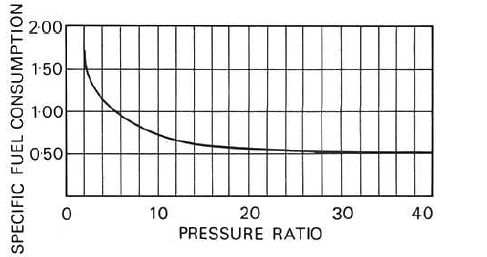
\includegraphics[width=0.5\textwidth]{consumovspressao}
    \caption{Specific Consumption.\cite{RollsRoyce}}
    \label{fig:consumovspressao}
\end{figure}


Using the \gls{LEAP}-1A \gls{HPC} as example, an axial compressor consists of one or more rotor assemblies which in turn can be one single part, representing a blisk, or a circumferential blade assembly. These assemblies are mounted between the 2 bearing in a casing which incorporate the stator vanes.

As mentioned in the previous sections, this compressor is a twin-spool, multi-stage unit consisting of 3+10 stages.

In other words, the compressor is composed of the \gls{LPC} with three stages, followed by the \gls{HPC} with ten stages. Additionally, the front fan can also be considered part of the compression system, as it contributes to air compression despite not being its primary function, effectively serving as the first stage of the \gls{LPC}.

\begin{figure}[H]
    \centering
    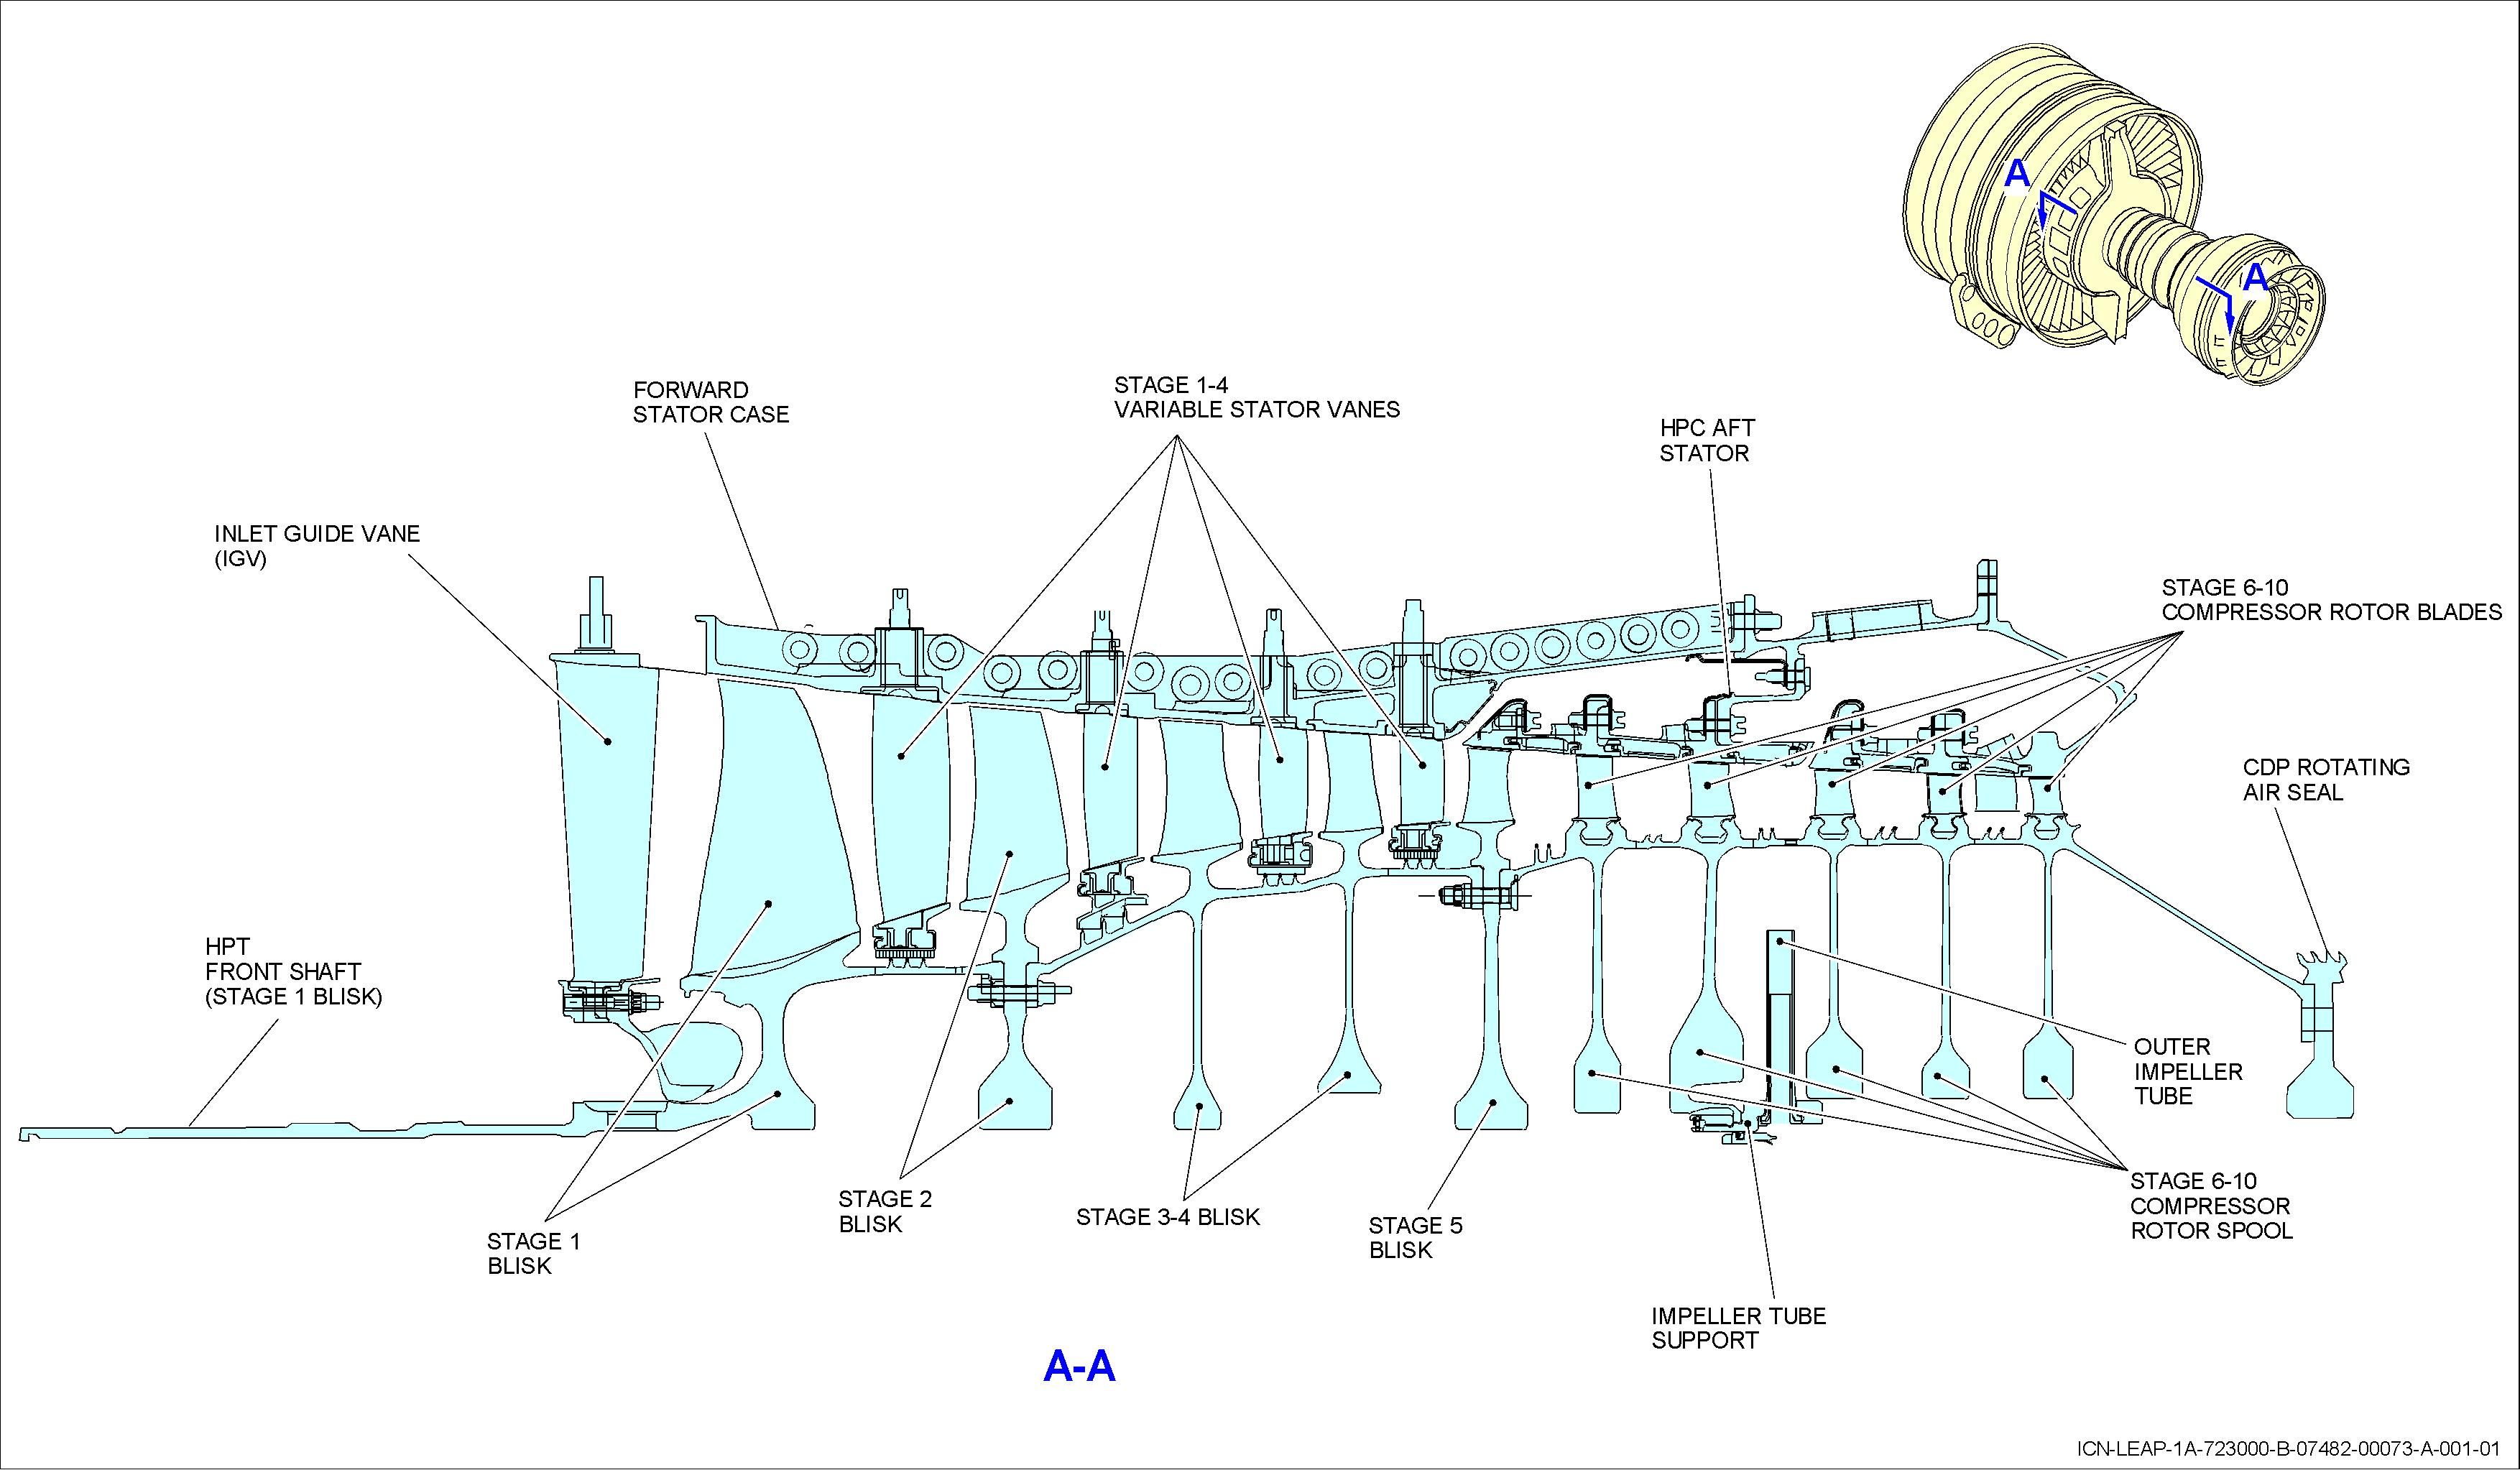
\includegraphics[width=0.8\textwidth]{hpc}
    \caption{LEAP-1A HPC.\cite{ESM}}
    \label{fig:hpc}
\end{figure}


With the engine running, the turbine transmits power to the compressor, driving it at high speed and ensuring a continuous airflow. As the air enters the \gls{LPC}, it passes through the first rotor, where the rotating airfoil-shaped blades transfer kinetic energy to the airflow by increasing its tangential momentum. Simultaneously, pressure rises with the aid of the diffusion process.
Next the air flows into the vanes  where kinetic energy increase is converted in pressure increase by the same process found in the rotationary step. 

The requirement for a high-pressure ratio on the shaft demands precise airflow control during engine operation to prevent airflow reversal, as a compressor inherently forces air from a low-pressure region to a higher-pressure zone. To achieve this, the guide vanes in the initial four stages functions as Variable Stator Vanes (VSV's), followed by fixed stator vanes in the subsequent stages. These variable vanes progressively close at lower airflow speeds to maintain an optimal air angle on the downstream rotor blades, preventing reverse flow and avoiding compressor stall.

During each stage the increase of pressure is relatevely small as shown in Figure~\ref{fig:graphcompressor} in order to avoid air breakaway at the blades and subsequent blade stall. On another hand, the multi-stage process alows the \gls{LEAP} to achieve an Overall Pressure ratio of 40:1. This ratio represents the Pressure ratio of all the engine not just the compressor. 

\begin{figure}[H]
    \centering
    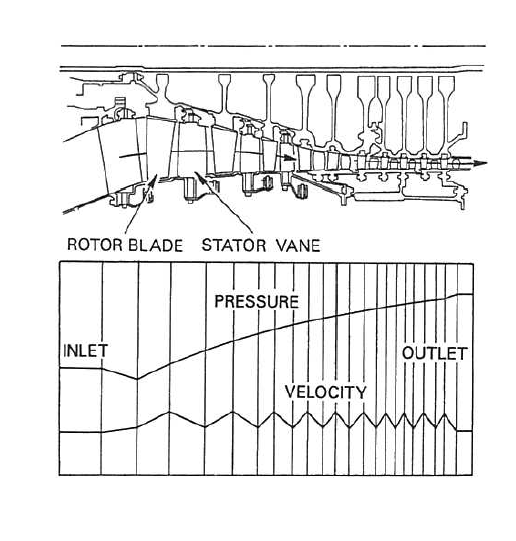
\includegraphics[width=0.5\textwidth]{graphcompressor}
    \caption{Axial Compressor Diagram and Pressure/Velocity Distribution.\cite{RollsRoyce}}
    \label{fig:graphcompressor}
\end{figure}

\section{Blisks vs Bladed disks}
\label{sec: blisks_disks}

In Figure~\ref{fig:blisks}, the \gls{HPC} of the \gls{LEAP}-1A engine is shown, consisting of five blisks, an impeller tube support, a five-stage rotor, and a rotating seal.

The incorporation of blisks in compressors represents a significant innovation in the \gls{LEAP}-1A design compared to previous-generation turbofan engines. This advancement was introduced in aviation to enhance engine performance. Blisks significantly reduce rotor weight compared to conventional aero-engine disks. Since compressor and turbine disks contribute to over 20\% of the engine's structural weight, their design presents numerous static and dynamic challenges.

From a design perspective, traditional bladed disks require the assembly of multiple components with different connection features, such as airfoil roots, disk roots, and locking mechanisms. In contrast, a blisk integrates all these elements into a single part, leading to several benefits:
\begin{itemize}
    \item A reduction in the total number of parts, contributing to lower overall weight and faster assembly.
    \item Fewer contact surfaces, minimizing gaps where airflow could infiltrate and disrupt engine operation.
    \item Eliminates dovetails and its associated issues such as its wheight and propensity for leakeges.
    \item Simplified assembly during both production and maintenance, resulting in lower manufacturing costs and shorter lead times.
    \item The use of blisks implie bigger clearence between the blade tip and the stator which impacts engines performance. 
\end{itemize}
However, blisks present significant drawbacks when compared to bladed disks, particularly in terms of maintenance and repairability. In the event of damage to an individual airfoil, the entire blisk must be replaced, leading to considerably higher costs than replacing a single blade. Additionally, as a single integrated component, the blisk eliminates the option of using different materials for the airfoil and the disk. The increased rigidity of the blisk also results in a lack of damping, which reduces its fatigue resistance.

\begin{figure}[H]
    \centering
    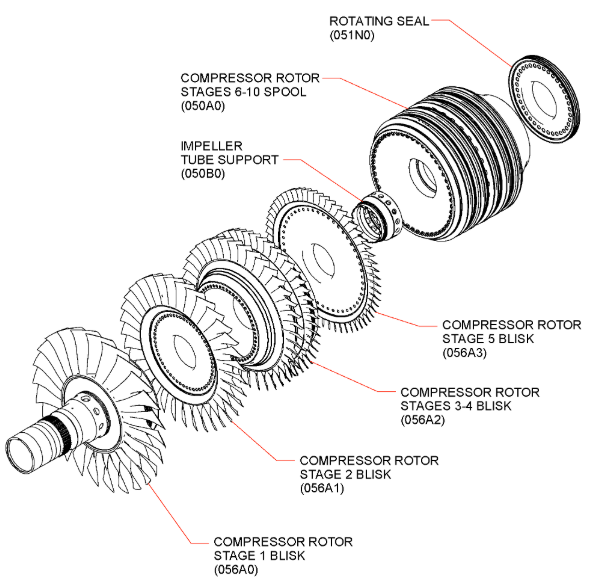
\includegraphics[width=0.8\textwidth]{blisks}
    \caption{LEAP-1A HPC. \cite{ESM}}
    \label{fig:blisks}
\end{figure}



\section{Rotor Blades}
\label{sec:blades_vanes}

As previously described, the \gls{HPC} of the \gls{LEAP}-1A consists of 10 stages, with the first five rotors designed as blisks and the last five as disks with fixed rotor blades. The attachment of these blades to the disk can be achieved through two different methods: axial or circumferential fixing, as illustrated in Figure~\ref{fig:fixings}.

\begin{figure}[H]
    \centering
    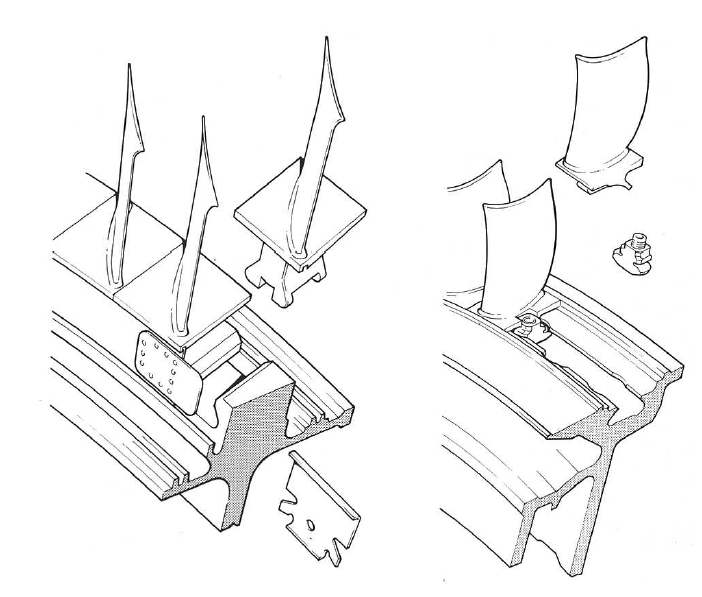
\includegraphics[width=0.5\textwidth]{fixings}
    \caption{Axial Fixing on the left and circumferential on the right.\cite{RollsRoyce}}
    \label{fig:fixings}
\end{figure}

The blades and disk shown in Figure~\ref{fig:fixings} are not actual \gls{LEAP}-1A components but merely illustrative examples.

The blades of the last five stages of the HPC are made from Inconel 718 and Inconel 718Plus. Inconel 718 is used in the first two stages, while Inconel 718Plus is used in stages 8, 9, and 10.

This material differs from the the blades found on the LPC or the blisks since with the increase of pressure temperature also rises. 

INCONEL alloy 718 (UNS N07718\texttt{/}W.Nr. 2.4668) is a high-strength, corrosion-resistant nickel chromium material used at \text{-}252.78 to 704.44\textdegree C.~\cite{inconel718}

Focusing on the last five stages of the HPC, in alignment with the objectives of this thesis, it is crucial to understand which dimensions impact the engine's performance, particularly as blade dimensions undergo changes due to excessive wear and usage, ultimately affecting engine performance and reliability.

TAP ME technicians are responsible for monitoring the most critical dimensions during the engine repair process.

These dimensions are specified in \cite{ESM} and are illustrated in Figure~\ref{fig:stage6}. Based on this, the critical dimensions can be defined as follows: tip chord length (CH), blade tip length (H), leading edge thickness (TL), and trailing edge thickness (TU).

\begin{figure}[H]
    \centering
    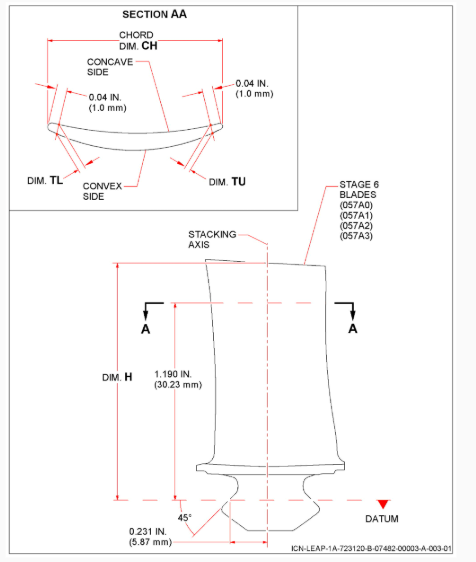
\includegraphics[width=0.5\textwidth]{stage 6}
    \caption{Stage 6 Blade Dimension Check.\cite{ESM}}
    \label{fig:stage6}
\end{figure}

In each stage of the HPC, the blades can be categorized into three types: narrow body blades, wide body blades, and locking blades. The narrow and wide body blades are used to adjust the platform gaps, ensuring proper assembly and optimal aerodynamic performance. The locking blades, on the other hand, incorporate locking mechanisms that secure them in place, preventing movement during engine operation. The correct selection and placement of these blade types are essential to maintaining structural integrity and performance within the compressor.
Therefore, ensuring the correct gap between the blades during the repair process is crucial to maintaining proper assembly, aerodynamic efficiency, and overall engine reliability.

\section{Degradation Mechanisms of Compressor Blades}
\label{sec:degradation}

The degradation of compressor blades is a critical factor affecting engine performance and reliability. Commercial aircraft engines operate in diverse environments, exposing the engine core to various particles and contaminants.

These ingested particles, collectively known as \gls{FOD}, include sand, metal fragments, birds, and other debris. The ingestion of such contaminants has two main consequences: if the particle is a hardbody, it can cause direct erosion and structural damage to the blades, leading to dimensional loss. In contrast, if the particle is a softbody, such as a bird, it can obstruct airflow, causing performance degradation or even severe engine failure.

In particular, this section examines the impacts of \gls{FOD} on the geometry of compressor blades. The ingestion of particles during the engine cycle can lead to a reduction in blade chord, loss of blade thickness, alteration of the leading and trailing edge shapes, thinning of the blade trailing edge, blunting of the leading edge, and an increase in surface roughness.

Alterations in the blade geometry, such as changes in chord length, thickness loss, and alterations to the leading and trailing edges, result in increased clearance losses at the blade tips, higher frictional losses, and a significant reduction in off-idle and open beta stall margins. In Figure~\ref{fig:leadedge} its possible to observe the damages caused on the leading edge by continuous erosion. \cite{Shi2023}

\begin{figure}[H]
    \centering
    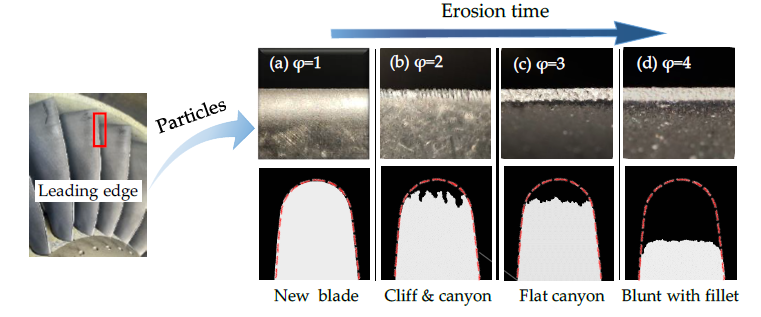
\includegraphics[width=0.8\textwidth]{leading edge}
    \caption{The effect on erosion trough time on the leading edge of a compressor blade \cite{Shi2023}}
    \label{fig:leadedge}
\end{figure}


These effects influence \gls{HPC} efficiency and, consequently, engine performance. In particular, compressor blade erosion, coupled with efficiency losses throughout the engine, can increase fuel consumption by nearly 1 percent compared to new blades (see Figure~\ref{fig:consumo_desgaste}) \cite{Shi2023}.

\begin{figure}[H]
    \centering
    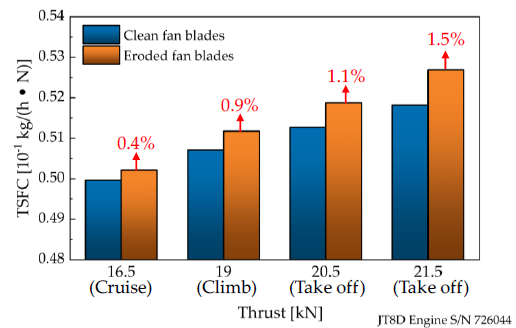
\includegraphics[width=0.6\textwidth]{consumo_desgaste}
    \caption{Comparison of thrust-specific fuel consumption (TSFC) between eroded and new compressor blades.\cite{Shi2023}}
    \label{fig:consumo_desgaste}
\end{figure}




